\documentclass[a4paper]{article}
\usepackage{import}
\usepackage{graphicx}
\usepackage{float}
\usepackage{pgfplots}
\usepackage{listings}
\usepackage{enumitem}
\usepackage{tikz}
\usetikzlibrary{decorations.pathreplacing} % for angle arc
\usetikzlibrary{angles, quotes, calc, positioning, trees} % for drawing angles
\pgfplotsset{compat=1.18,width=10cm}
\usepackage{tikz-cd}
\usepackage{booktabs}
\usepackage{cancel}
\usepackage{amsmath}
\usepackage{csquotes}
\usepackage{gensymb}
\usepackage{forest}
\usepackage{amsthm}
\usepackage{amssymb}
\usepackage{pgfplots}
\usepackage{lipsum}
\usepackage{mdframed} 
\usepackage{color}   
\usepackage{hyperref}
\newmdtheoremenv{theo}{Theorem}
\usepackage{mathtools}
\DeclarePairedDelimiter\ceil{\lceil}{\rceil}
\DeclarePairedDelimiter\floor{\lfloor}{\rfloor}

\hypersetup{
    colorlinks=true, %set true if you want colored links
    linktoc=all,     %set to all if you want both sections and subsections linked
    linkcolor=black,  %choose some color if you want links to stand out
}

% Define theorem styles
\newtheorem{theorem}{Theorem}[section]    % Theorems numbered within sections
\newtheorem{lemma}[theorem]{Lemma}        % Lemmas use the same counter as theorems
\newtheorem{corollary}[theorem]{Corollary} % Corollaries use the same counter as theorems
\newtheorem{proposition}[theorem]{Proposition} % Proposition uses the same counter
\newtheorem{property}[theorem]{Property}
\theoremstyle{definition}
\newtheorem{definition}[theorem]{Definition} % Now uses the same counter as theorems


% Remark-style theorem
\theoremstyle{remark}
\newtheorem{remark}[theorem]{Remark}

% Boxed environment for theorems
\newmdenv[
  linewidth=0.8pt,
  roundcorner=5pt,
  linecolor=black,
  backgroundcolor=white!5,
  skipabove=\baselineskip,
  skipbelow=\baselineskip,
  innerleftmargin=10pt,
  innerrightmargin=10pt,
  innertopmargin=5pt,
  innerbottommargin=5pt
]{thmbox}

% Custom proof environment (also boxed)
\renewenvironment{proof}[1][Proof]{%
  \begin{mdframed}[linewidth=0.8pt, roundcorner=5pt, linecolor=black, skipabove=\baselineskip, skipbelow=\baselineskip, innertopmargin=5pt, innerbottommargin=5pt]%
  \noindent\textbf{#1. }%
}{%
  \end{mdframed}%
}

% Redefine theorem environments to use thmbox
\let\oldtheorem\theorem
\renewenvironment{theorem}{\begin{thmbox}\begin{oldtheorem}}{\end{oldtheorem}\end{thmbox}}

\let\oldlemma\lemma
\renewenvironment{lemma}{\begin{thmbox}\begin{oldlemma}}{\end{oldlemma}\end{thmbox}}

\let\oldcorollary\corollary
\renewenvironment{corollary}{\begin{thmbox}\begin{oldcorollary}}{\end{oldcorollary}\end{thmbox}}

\let\oldproposition\proposition
\renewenvironment{proposition}{\begin{thmbox}\begin{oldproposition}}{\end{oldproposition}\end{thmbox}}

\let\oldproperty\property
  \renewenvironment{property}{\begin{oldproperty}}{\end{oldproperty}}


% Reference shortcuts
\newcommand{\thmref}[1]{Theorem~\ref{#1}}
\newcommand{\lemref}[1]{Lemma~\ref{#1}}
\newcommand{\corref}[1]{Corollary~\ref{#1}}
\newcommand{\propref}[1]{Property~\ref{#1}} 

% To customize QED symbol
\renewcommand{\qedsymbol}{$\blacksquare$}

\usetikzlibrary{decorations.pathreplacing} % for angle arc
\usetikzlibrary{angles, quotes, calc} % for drawing angles

\usepackage{color}   %May be necessary if you want to color links
\usepackage{hyperref}
\hypersetup{
    colorlinks=true, %set true if you want colored links
    linktoc=all,     %set to all if you want both sections and subsections linked
    linkcolor=black,  %choose some color if you want links to stand out
}

\usepackage{xcolor}
\usepackage[most]{tcolorbox}
% Define a custom tcolorbox environment for examples
\newtcolorbox{examplebox}[2][]{
  colback=blue!5!white,
  colframe=blue!30!black,
  title=#2,
  boxrule=0mm,
  fonttitle=\bfseries,
  width=\textwidth,
  breakable,
  #1
}

\newtcolorbox{definizione}[2] {
  colback=green!5!white,
  colframe=green!30!black,
  title=#2,
  boxrule=0mm,
  fonttitle=\bfseries,
  width=\textwidth,
  breakable,
  #1
}

\definecolor{codegreen}{rgb}{0,0.6,0}
\definecolor{codegray}{rgb}{0.5,0.5,0.5}
\definecolor{codepurple}{rgb}{0.58,0,0.82}
\definecolor{backcolour}{rgb}{0.95,0.95,0.92}

\lstdefinestyle{mystyle}{
    backgroundcolor=\color{backcolour},   
    commentstyle=\color{codegreen},
    keywordstyle=\color{magenta},
    numberstyle=\tiny\color{codegray},
    stringstyle=\color{codepurple},
    basicstyle=\ttfamily\footnotesize,
    breakatwhitespace=false,         
    breaklines=true,                 
    captionpos=b,                    
    keepspaces=true,                 
    numbers=left,                    
    numbersep=5pt,                  
    showspaces=false,                
    showstringspaces=false,
    showtabs=false,                  
    tabsize=2
}

\lstset{style=mystyle}

\makeatletter
\renewcommand*\env@matrix[1][*\c@MaxMatrixCols c]{%
  \hskip -\arraycolsep
  \let\@ifnextchar\new@ifnextchar
  \array{#1}}
\makeatother


\onehalfspacing
\title{Basi di dati}
\author{Università di Verona\\Imbriani Paolo - VR500437\\Professor Alberto Belussi}

\begin{document}

\begin{figure}
    \centering
    \includegraphics[width=0.3\textwidth]{../UniversityofVerona.png}
    \label{fig:centered-image}
\end{figure}

\maketitle

\pagebreak

\tableofcontents

\pagebreak

\section{Introduzione}


Il corso si dividerà in Teoria al primo semestre e 
Tecnologie delle basi di dati e laboratorio al secondo semestre.
Questo modulo ha lo scopo di fornire allo studente conoscenze necessarie per la progettazione,
gestione e interrogazione di una \textit{base di dati}.
Competenze da acquisire da parte dello studente:
\begin{itemize}
    \item Progettazione concettuale di una base di dati e successiva implementazione dellla stessa sui più diffusi
    sistemi per la gestione di basi di dati
    \item interrogazione di una base di dati relazionale in algebra relazionale e calcolo relazionale
\end{itemize}

\section{Progettazione di una base di dati}
Il ciclo di vita di un processo di automazione di un sistema informativo è diviso in diverse
fasi:
\begin{itemize}
  \item \textbf{Studio di fattibilità}: si valuta se l'automazione del sistema
    informativo è possibile e conveniente
  \item \textbf{Raccolta e analisi dei requisiti}: si individuano proprietà e funzionalità
    del sistema (dati e applicazioni) producendo una descrizione completa ma informale
  \item \textbf{Progettazione}: si produce una descrizione formale del sistema
    informativo
\end{itemize}
La progettazione si divide in due parti principali che vanno di pari passo:
\begin{itemize}
  \item \textbf{Progettazione dei dati}: si produce una descrizione formale dei dati
    (schema). Una volta progettati i dati vengono implementati in un DBMS
  \item \textbf{Progettazione delle applicazioni}: si produce una descrizione formale
    delle applicazioni (specifica)
\end{itemize}
Una volta implementati i dati e le applicazioni si passa alla fase di \textbf{validazione
e collaudo}

\subsection{Progettazione dei dati}
Una metodologia di progettazione dei dati è costituita da:
\begin{itemize}
  \item \textbf{Decomposizione}: dividere in passi le attività di progetto
  \item \textbf{Strategie}: individuare un insieme di strategie e criteri di scelta da
    seguire
  \item \textbf{Modelli di riferimento}: utilizzare modelli di dati e tecniche di
    progettazione consolidate
\end{itemize}
Una buona metodologia deve essere:
\begin{itemize}
  \item Generale
  \item Facile da usare
  \item Deve produrre un risultato di qualità
\end{itemize}

\subsection{Requisiti}
\subsubsection{Progettazione concettuale}
La progettazione concettuale è la prima fase della progettazione dei dati. Lo scopo è
quello di produrre una descrizione formale dei dati (schema concettuale). Lo schema
deve essere \textbf{indipendente dall'implementazione}.

\vspace{1em}
\noindent
Non è solo un progetto intermedio, ma costituisce anche una porzione del risultato finale
perchè rappresenta una descrizione di \textbf{alto livello} del contenuto della base di
dati, comprensibile anche per utenti poco esperti.

\subsubsection{Progettazione logica}
La progettazione logica è la seconda fase della progettazione dei dati. Lo scopo è
quello di tradurre lo schema concettuale in uno schema logico in modo da poterlo
utilizzare su un sistema specifico. Lo schema logico infatti è dipendente dalle
tecnologie utilizzate. Bisogna tenere anche in considerazione le operazioni più
frequenti che le applicazioni effettueranno sulla base di dati.

\subsubsection{Progettazione fisica}
La progettazione fisica è la terza fase della progettazione dei dati. L'obiettivo è quello
di ottimizzare l'accesso ai dati completando lo schema logico con i parametri relativi
alla memorizzazione fisica dei dati e con gli opportuni metodi d'accesso (\textbf{indici}).

\section{Modello Entità-Relazione}
È un modello, formale e non ambiguo, utilizzato per la progettazione concettuale di una
base di dati. Fornisce strumenti formali (costrutti), con sintassi grafica, per specificare la
struttura e le proprietà dei dati da rappresentare indipendentemente dalla tecnologia.

\vspace{1em}
\noindent
Ogni costrutto viene definito specificando:
\begin{itemize}
  \item Il suo significato (o semantica)
  \item La sua sintassi grafica
  \item La rappresentazione delle sue istanze (o occorrenze)
\end{itemize}

\vspace{1em}
\noindent
Progettare indipendentemente dalle tecnologie significa:
\begin{itemize}
  \item \textbf{Non considerare} eventuali ottimizzazioni
  \item \textbf{Considerare} tutti i requisiti senza semplificazioni o convenzioni
  \item \textbf{Considerare} sempre i processi di generazione e modifica dei dati
    per verificare che ogni situazione sia rappresentabile da un'istanza "pulita"
    della base di dati
\end{itemize}

\subsection{Entità}
Un'entità \( E \) rappresenta una \textbf{classe di oggetti} che hanno le seguenti
caratteristiche:
\begin{itemize}
  \item \textbf{Proprietà comuni}
  \item \textbf{Eistenza autonoma} rispetto ad altre classi di oggetti
  \item \textbf{Identificazione univoca}, cioè esiste una chiara corrispondenza tra
    gli oggetti istanze di entità e concetti istanziati nel sistema informativo
\end{itemize}
Un entità si rappresenta con un rettangolo che contiene il nome dell'entità:
\begin{figure}[H]
  \centering
  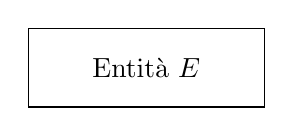
\begin{tikzpicture}
    \node[draw, rectangle, minimum width=3cm, minimum height=1cm ]
      (E) {Entità \( E \)};
  \end{tikzpicture}
  \caption{Rappresentazione grafica di un'entità}
\end{figure}

\subsubsection{Istanza}
Un'istanza dell'entità \( E \) è un \textbf{oggetto} appartenente alla classe rappresentata
da \( E \). Si indica con \( I(E) \) l'insieme delle istanze di \( E \) che esistono
nella base di dati in un certo istante e alla creazione della base di dati è vuota:
\( I(E) = \emptyset \).

\ex{}
{
  Rappresentiamo con il costrutto entità il concetto di \textbf{persona}. Bisogna gestire
  nella base di dati le informazioni che descrivono un gruppo di persone.
  \begin{figure}[H]
    \centering
    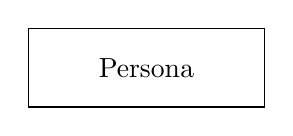
\begin{tikzpicture}
      \node[draw, rectangle, minimum width=3cm, minimum height=1cm ]
        (E) {Persona};
    \end{tikzpicture}
    \caption{Rappresentazione grafica dell'entità Persona}
  \end{figure}
  L'insieme delle istanze dell'entità Persona è il seguente:
  \[
    I(\text{Persona}) = \{p_1, p_2, p_3, \ldots\}
  \]
}

\subsection{Relazione}
Una relazione \( R \) rappresenta un \textbf{legame logico} tra \textbf{due o più} entità.
Può esserci anche una relazione all'entità stessa (relazione ricorsiva).

\vspace{1em}
\noindent
Una relazione si rappresenta nello schema con un rombo a cui si collegano attraverso delle
linee le entità coinvolte nella relazione. Il nome della relazione viene scritto a fianco
al rombo:
\begin{figure}[H]
  \centering
  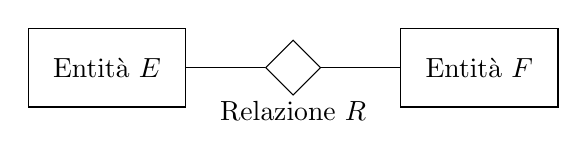
\begin{tikzpicture}
    \node[draw, rectangle, minimum width=2cm, minimum height=1cm ]
      (E1) {Entità \( E \)};
    \node[draw, diamond, minimum width=0.7cm, minimum height=0.7cm, right=1cm of E1]
      (R) {};
    \node[below=0.3cm] at (R) {Relazione \( R \)};
    \node[draw, rectangle, minimum width=2cm, minimum height=1cm, right=1cm of R]
      (E2) {Entità \( F \)};
    \draw (E1) -- (R);
    \draw (E2) -- (R);
  \end{tikzpicture}
  \caption{Rappresentazione grafica di una relazione tra due entità}
\end{figure}

\subsubsection{Istanza}
Data una relazione \( R \) tra \( n \) entità \( E_1, \ldots, E_n \) un'istanza della
relazione \( R \) è una \textbf{ennupla di istanze di entità}:
\[
  (e_1, \ldots, e_n) \; \text{dove } e_i \in I(E_i) \text{ per } 1 \le i \le n
\] 
La popolazione di \( R \) rappresenta l'insieme delle coppie di istanze delle entità
\( E \) e \( F \) che sono in relazione in un certo istante:
\[
  I(R) = \left\{ (e_i, f_j) \;\left|\; e_i \in I(E), f_j \in I(F) \right.\right\} 
\]
\ex{}
{
  Supponiamo che nello schema ci siano le entità \textbf{Persona} e \textbf{Comune},
  bisogna gestire la \textbf{Residenza} delle persone nei comuni italiani.

  \begin{figure}[H]
    \centering
    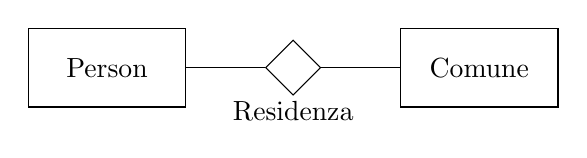
\begin{tikzpicture}
      \node[draw, rectangle, minimum width=2cm, minimum height=1cm ]
        (E1) {Person};
      \node[draw, diamond, minimum width=0.7cm, minimum height=0.7cm, right=1cm of E1]
        (R) {};
      \node[below=0.3cm] at (R) {Residenza};
      \node[draw, rectangle, minimum width=2cm, minimum height=1cm, right=1cm of R]
        (E2) {Comune};
      \draw (E1) -- (R);
      \draw (E2) -- (R);
    \end{tikzpicture}
    \caption{Rappresentazione grafica della relazione Residenza}
  \end{figure}
  \noindent
  Ciò implica che per esistere un'istanza di residenza devono esistere un'istanza
  di persona e un'istanza di comune.
}
Data una relazione \( R \) tra \( n \) entità \( \{E_1, E_2, \ldots, E_n\} \)
vale \textbf{sempre} la seguente proprietà sull'insieme delle istanze \( I(R) \):
\[
  I(R) \subseteq I(E_1) \times I(E_2) \times \ldots \times I(E_n)
\] 
La conseguenza di questa proprietà è che non è possibilie rappresentare la stessa ennupla
più volte.

\subsubsection{Relazione ricorsiva}
È una relazione binaria sulla stessa entità:
\begin{figure}[H]
  \centering
  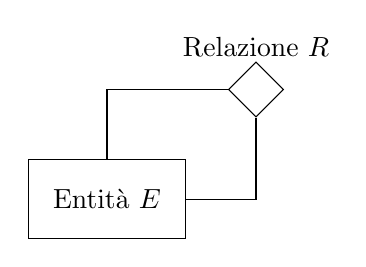
\begin{tikzpicture}
    \node[draw, rectangle, minimum width=2cm, minimum height=1cm ]
      (E) {Entità \( E \)};
    \node[draw, diamond, minimum width=0.7cm, minimum height=0.7cm, above right=1cm of E]
      (R) {};
    \node[above=0.3cm] at (R) {Relazione \( R \)};

    \draw (E) |- (R);
    \draw (E) -| (R);
  \end{tikzpicture}
  \caption{Rappresentazione grafica di una relazione ricorsiva}
\end{figure}

\subsection{Attributo}
Rappresenta una proprietà elementare di un'entità o di una relazione.
Ogni attributo di un'entità o di una relazione associa ad ogni istanza \textbf{un solo}
valore appartenente ad un dominio di valori ammissibili. Può essere visto
come una funzione che ha come dominio le istanze dell'entità (o relazione) e come
codominio l'insieme dei valori ammissibili:
\[
  f_A: I(E) \mapsto D
\] 
dove \( a \) è un attributo dell'entità \( E \), mentre \( I(E) \) l'insieme delle
istanze di \( E \) e \( D \) è l'insieme dei valori ammissibili.

\vspace{1em}
\noindent
La sintassi grafica di un attributo è un cerchio \textbf{vuoto} collegato con una linea all'entità
con accanto il nome dell'attributo:
\begin{figure}[H]
  \centering
  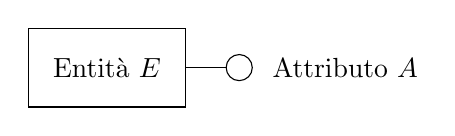
\begin{tikzpicture}
    \node[draw, rectangle, minimum width=2cm, minimum height=1cm ]
      (E) {Entità \( E \)};
    \node[draw, circle, right=0.5cm of E]
      (A) {};
    \node[right=0.3cm] at (A) {Attributo \( A \)};
    \draw (E) -- (A);
  \end{tikzpicture}
  \caption{Rappresentazione grafica di un attributo di un'entità}
\end{figure}

\begin{figure}[H]
  \centering
  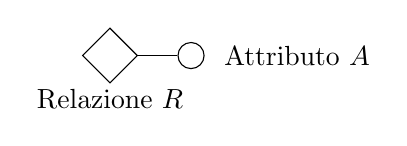
\begin{tikzpicture}
    \node[draw, diamond, minimum width=0.7cm, minimum height=0.7cm ]
      (E) {};
    \node[below=0.3cm] at (E) {Relazione \( R \)};
    \node[draw, circle, right=0.5cm of E]
      (A) {};
    \node[right=0.3cm] at (A) {Attributo \( A \)};
    \draw (E) -- (A);
  \end{tikzpicture}
  \caption{Rappresentazione grafica di un attributo di una relazione}
\end{figure}

\ex{}
{
  Rappresentiamo il concetto di persona tramite un'entità, bisogna gestire nella base
  di dati il nome e il cognome di un gruppo di persone.
  \begin{figure}[H]
    \centering
    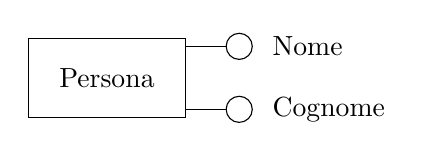
\begin{tikzpicture}
      \node[draw, rectangle, minimum width=2cm, minimum height=1cm ]
        (E) {Persona};
      \node[draw, circle, yshift=0.4cm, right=0.5cm of E]
        (A1) {};
      \node[right=0.3cm] at (A1) {Nome};
      \node[draw, circle, yshift=-0.4cm, right=0.5cm of E]
        (A2) {};
      \node[right=0.3cm] at (A2) {Cognome};
      \draw (A1) -- +(-0.68cm,0);
      \draw (A2) -- +(-0.68cm,0);
    \end{tikzpicture}
    \caption{Rappresentazione grafica dell'entità Persona con gli attributi Nome e Cognome}
  \end{figure}
}






\end{document}